
\section{Results}

\subsection{CC efficiency}

	\begin{figure} [!hbtp]	
	\centering
	\caption{Detection efficiency function of the Compton Camera position.}	
	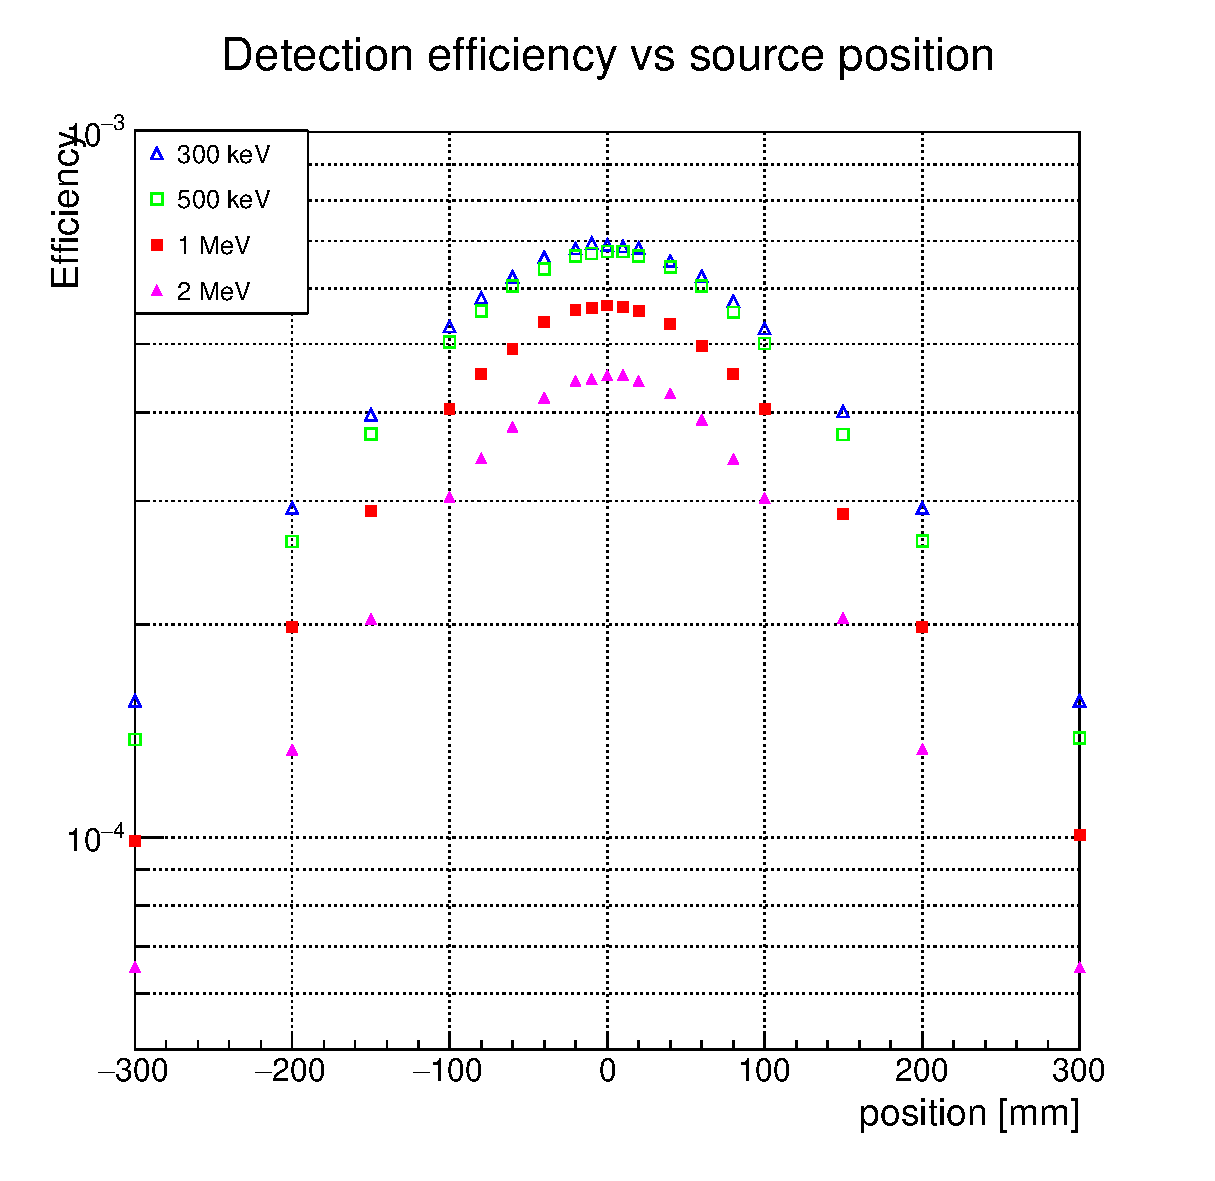
\includegraphics[width=0.7\textwidth]{./Figure/2017-06-26_Efficiency_CC_articles.eps}
	\end{figure}


\subsection{Beam intensity }
Je traite les simulations pour une statistique de $10^{8}$ pour les protons et une statistique de $2\times10^{5}$ pour les ions carbone.\newline
J'assigne à chaque particule interagissant dans le diffuseur et l'absorbeur un num\'ero de paquet auquel elle est th\'eoriquement rattach\'ee au vu de la structure en temps choisie et de l'intensit\'e du faisceau.
The modification of the beam intensity will change the number of particles included in a bunch. For instance, at the clinical intensity in protons, there is in average 217 protons in a bunch.



The beam intensity plays an important role for the Compton camera concerning its capability to distinct events in coincidence. In the simulation, the beam intensity is modeled by an average number of particles per bunch. The exact number of particles in each bunch is given by a random draw in a Poisson distribution, where the mean value is the beam intensity chosen. The range of intensities was chosen in order to cover almost all the possibilities: from a very low beam intensity to the clinical beam intensity. Therefore, for proton and carbon ion, the lowest beam intensity is set to 0.001 particles per bunch in average and for protons goes up to 217 protons per bunch when in case of carbon ion, it goes up to 70 particles per bunch. The coincidence yields are scaled per ion incidents and the beam intensity per average ions per bunch. The true coincidences represent a coincidence in the camera by the same gamma ray. The background corresponds to all the other coincidence types.


\begin{figure} [!h]
\caption{Coincidences yield for protons (a) and carbon ions (b) in function of the beam intensity. The intensity is given for a number of incident particles per bunch.  The distinction between the filled markers and the empty ones are that the time of flight discrimination is applied in the case of empty markers.}
\subfloat[]{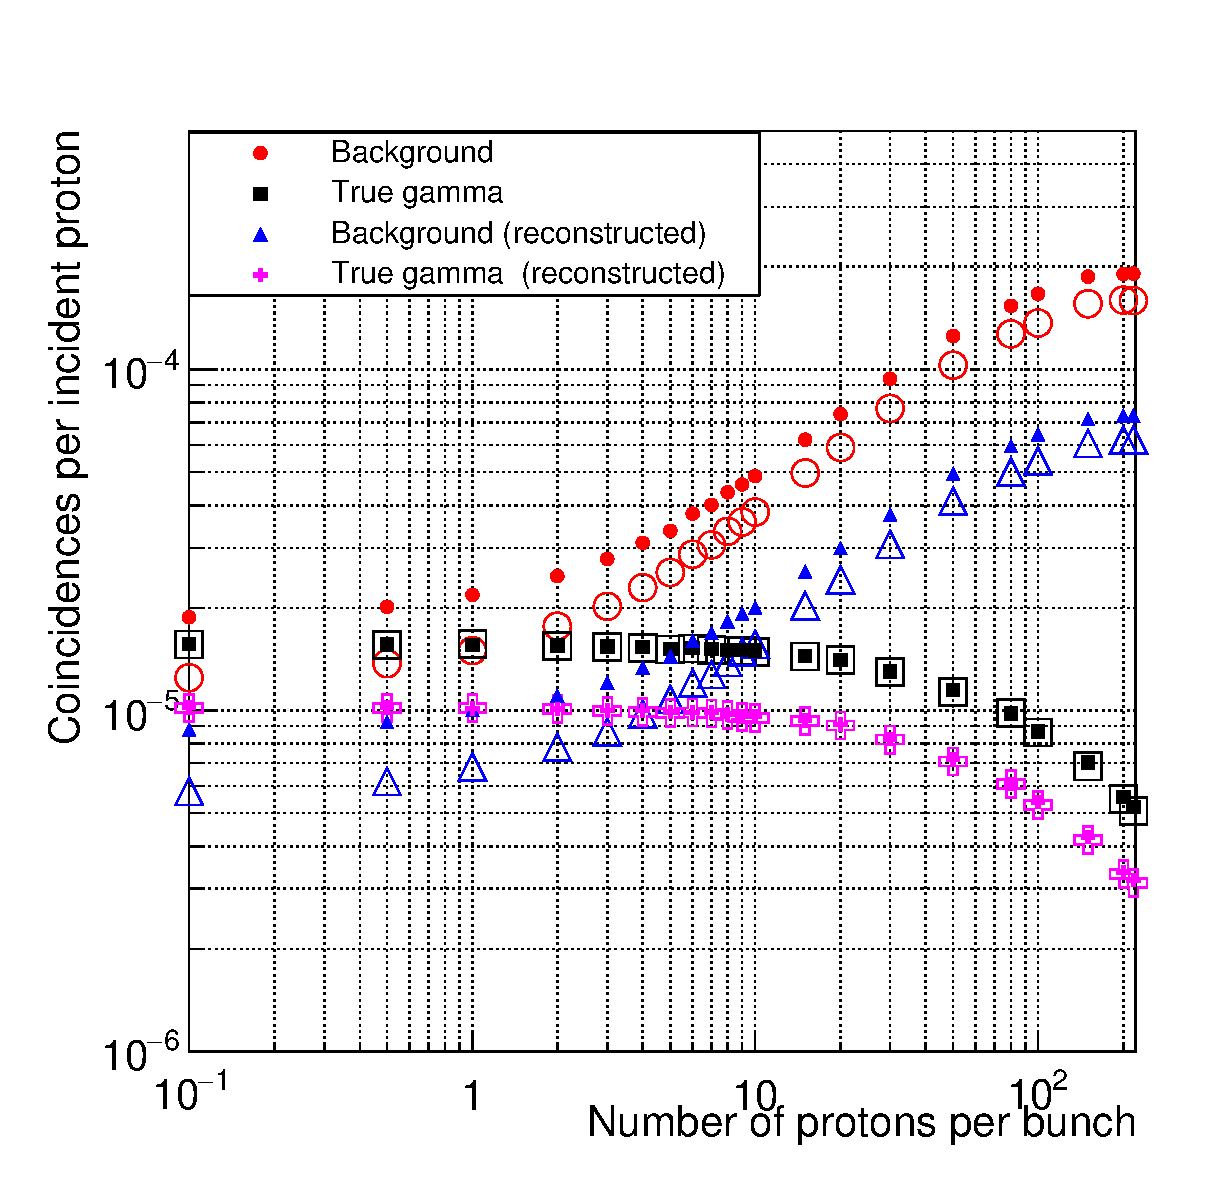
\includegraphics[width=0.5\textwidth]{./Figure/2017_06_28_Taux_coincidences_variation_protons_New_design_4EntreesLegend_LogXLogY.eps}}
 \subfloat[]{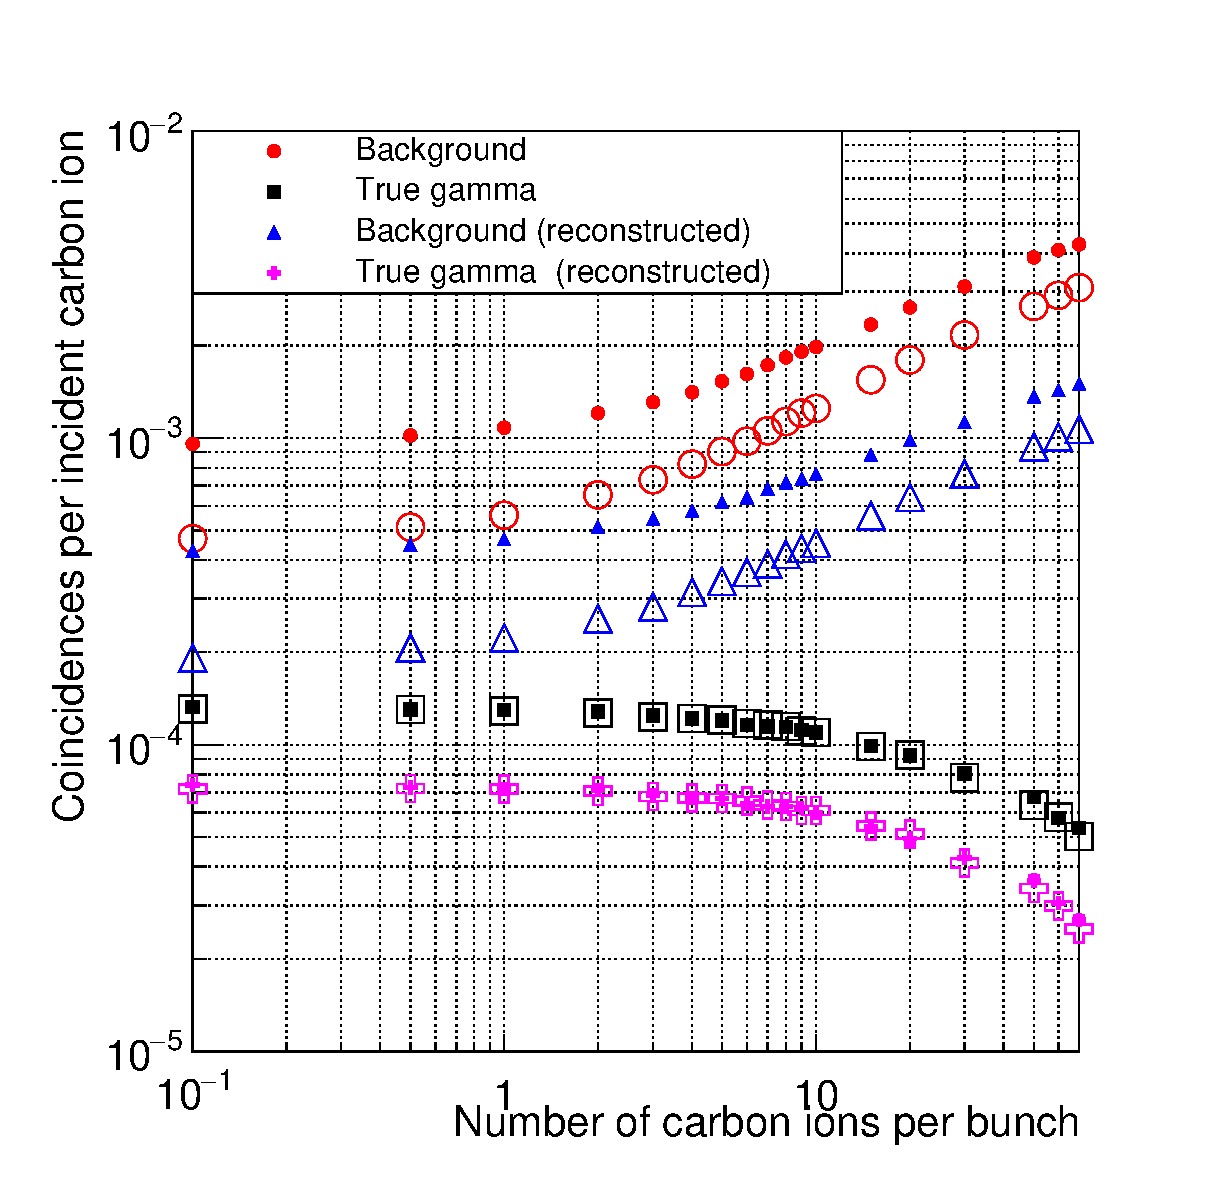
\includegraphics[width=0.5\textwidth]{./Figure/2017_06_28_Taux_coincidences_variation_carbonIons_New_design_4EntreesLegend_LogXLogY.eps}}
  \label{fig:coincidences}
\end{figure}

\newpage
At the clinical beam intensity, the high background level is mainly due to the random coincidences. In fact, the probability to detect two radiation coming from two different incident particles increases with the number of incident particles per bunch. Another issue is the single rate of events detected by each detector at those high intensities. For instance, at the clinic beam intensity in proton therapy, the single rate on the absorber is around 300 MHz and on the first silicon layer it is around 20 MHz. The current electronic front end and acquisition system are not able to treat this amount of data coming from all the detectors. As a result, it appears that it is impossible to use the Compton camera at a clinical beam intensity for the treatment monitoring in ion therapy.\newline
Nevertheless, if the intensity decreases enough to avoid almost all the random coincidences, the monitoring seems more feasible. In addition, it can be supposed that the time of flight discrimination will improve the signal to the background ratio at low intensities by suppressing the coincidences induced by charged particles. Indeed, the charged particles are slower than gamma rays which move at the light speed.\newline

\subsection{Comparaison LM-MLEM vs Line cone reconstruction}


\begin{figure} [!h]
\subfloat[]{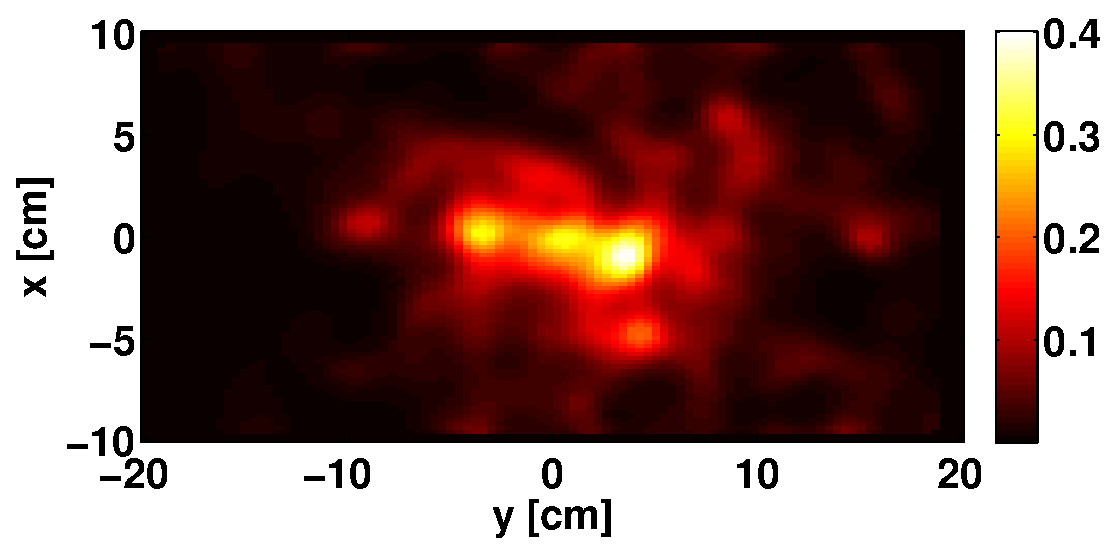
\includegraphics[width=0.5\textwidth]{./Figure/MLEM_2D.pdf}}
 \subfloat[]{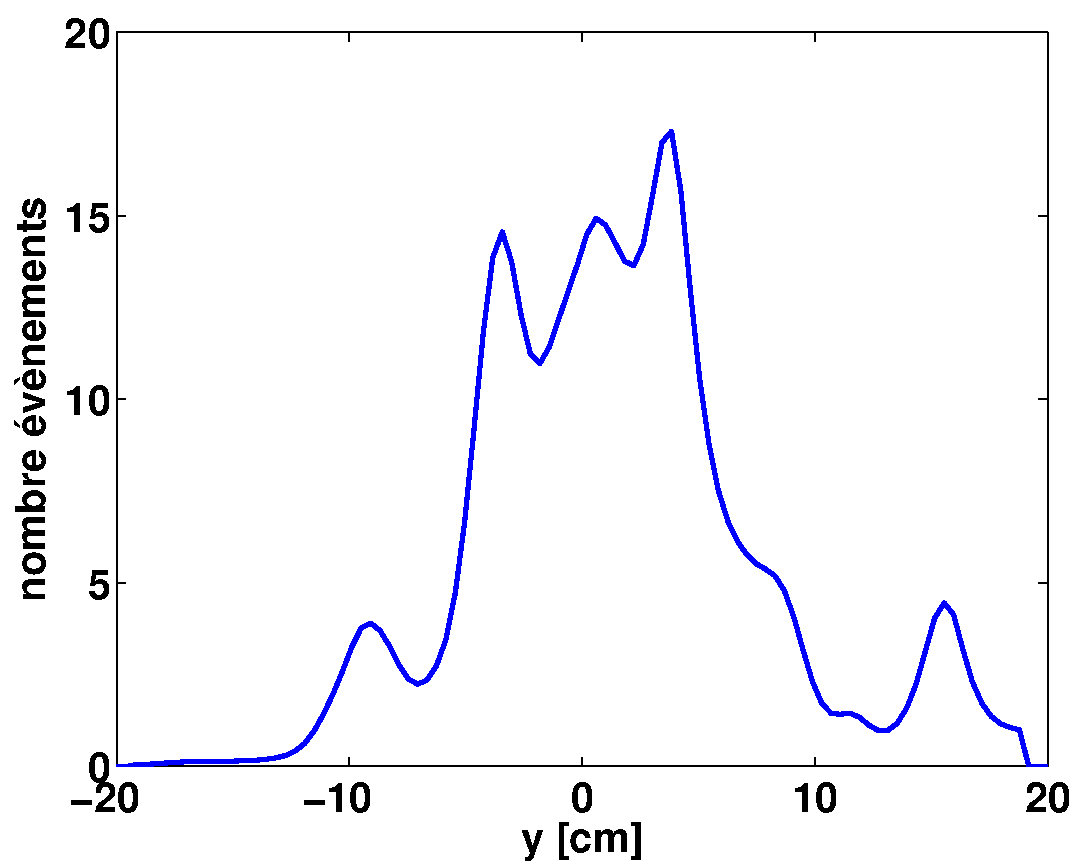
\includegraphics[width=0.5\textwidth]{./Figure/MLEM_1D.pdf}}\\
  \subfloat[]{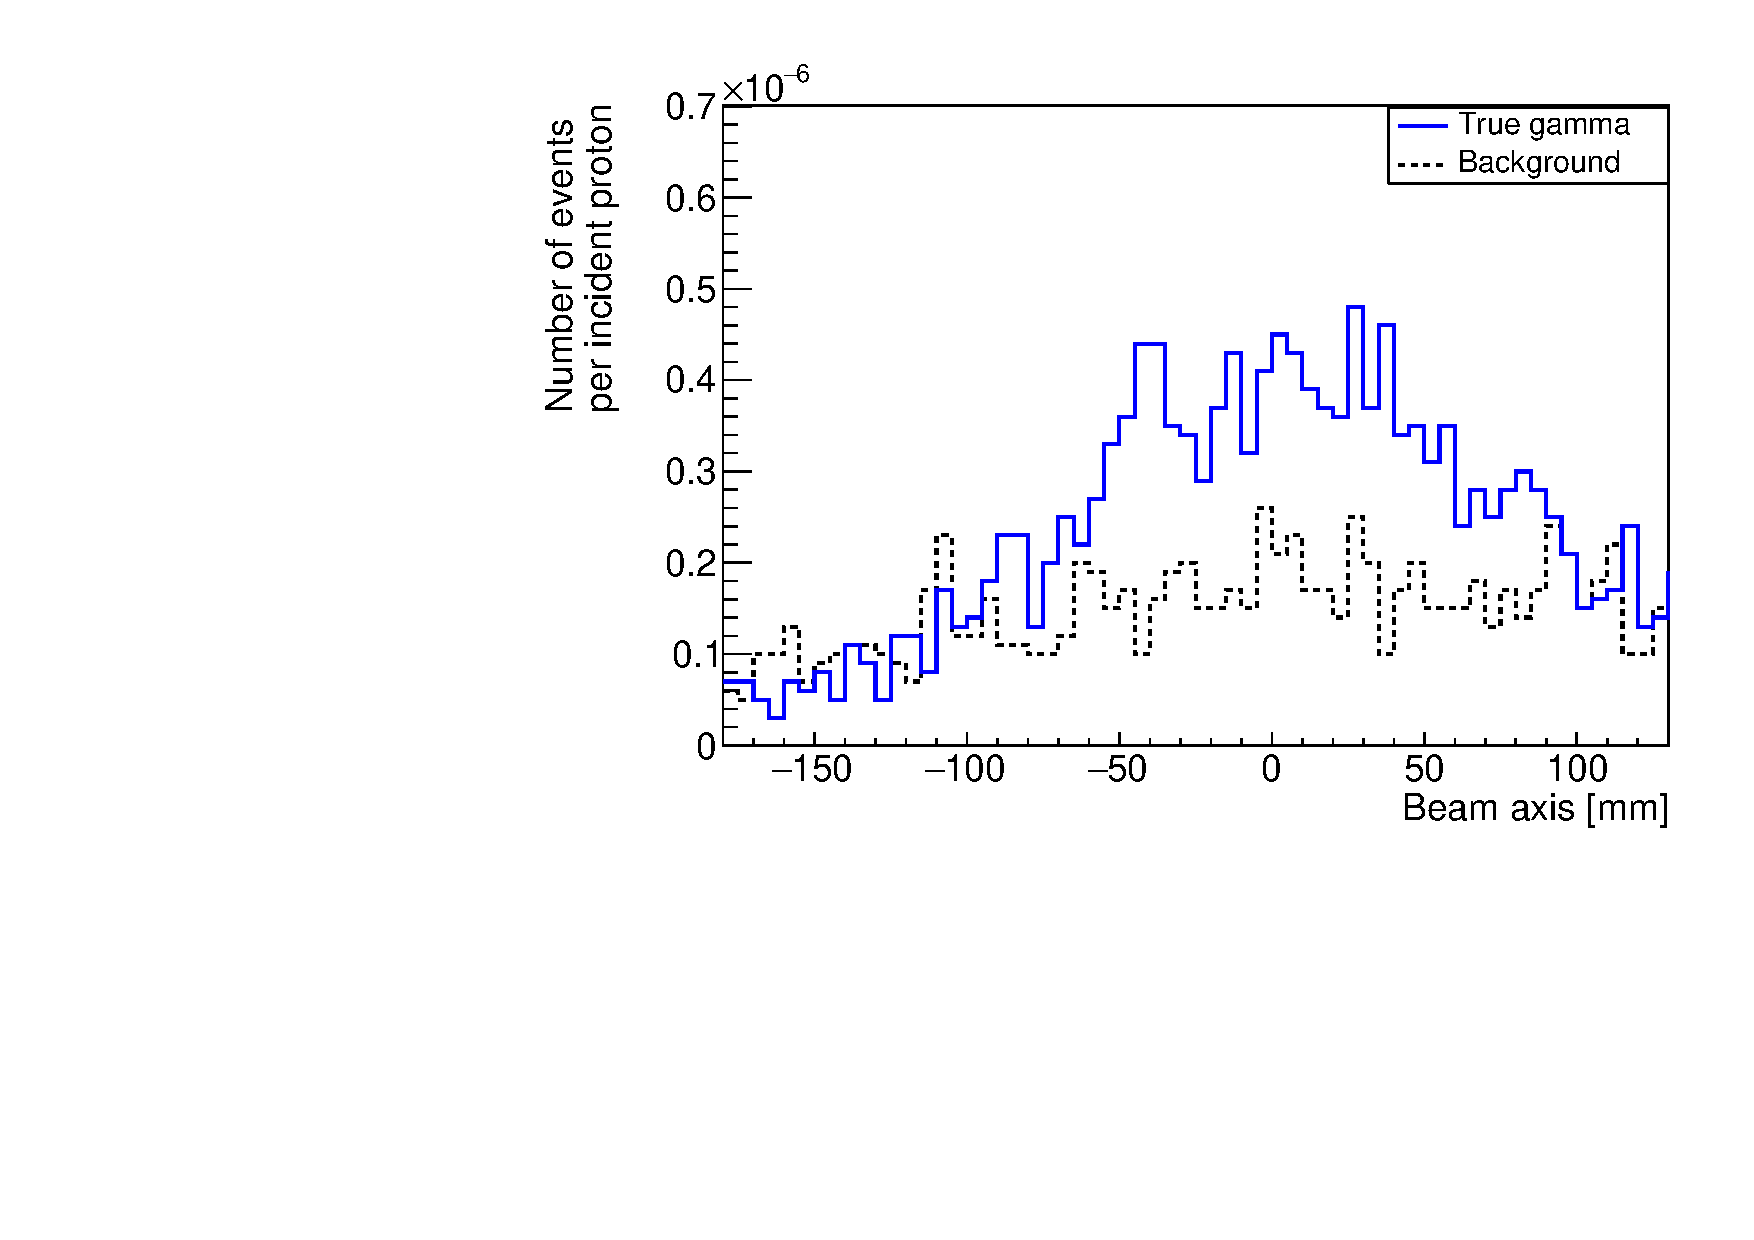
\includegraphics[width=0.5\textwidth]{./Figure/2015_02_16_Reconstruction_coinc_160MeVProton_TOF_6ns_file0to100_zoom.pdf}}
  \label{fig:comparaison}
  \caption{Comparaison LM-MLEM vs Line cone reconstruction}

\end{figure}

%   \begin{verbatim}
% a) 2015_10_20_Volume_100x100x5_voxels_and_size_20x40x1_source_Proton160MeV_camera_50mm_stat_2175events_sans_MatriceSensibility_bordYplusmoins-3_bordXplusmoins-3_median_iteration_10.
% b) 2015_10_20_Volume_100x100x5_voxels_and_size_20x40x1_source_Proton160MeV_camera_50mm_stat_2175events_sans_MatriceSensibility_bordYplusmoins-3_bordXplusmoins-3_selectionX_20mm_Filtre_median_iteration_Profil_Y_iteration_10. 
% c)  2015_02_16_Reconstruction_coinc_160MeVProton_TOF_6ns_file0to100_zoom               
%  \end{verbatim}

\subsection{Compton camera precision}


The information given by a control device as the Compton camera has to be viable and as precise as possible. In order to estimate the precision of the Compton camera, a method is used. 

\begin{figure}[!hbtp]	
\centering
\caption{Precision function of the incident protons .}	
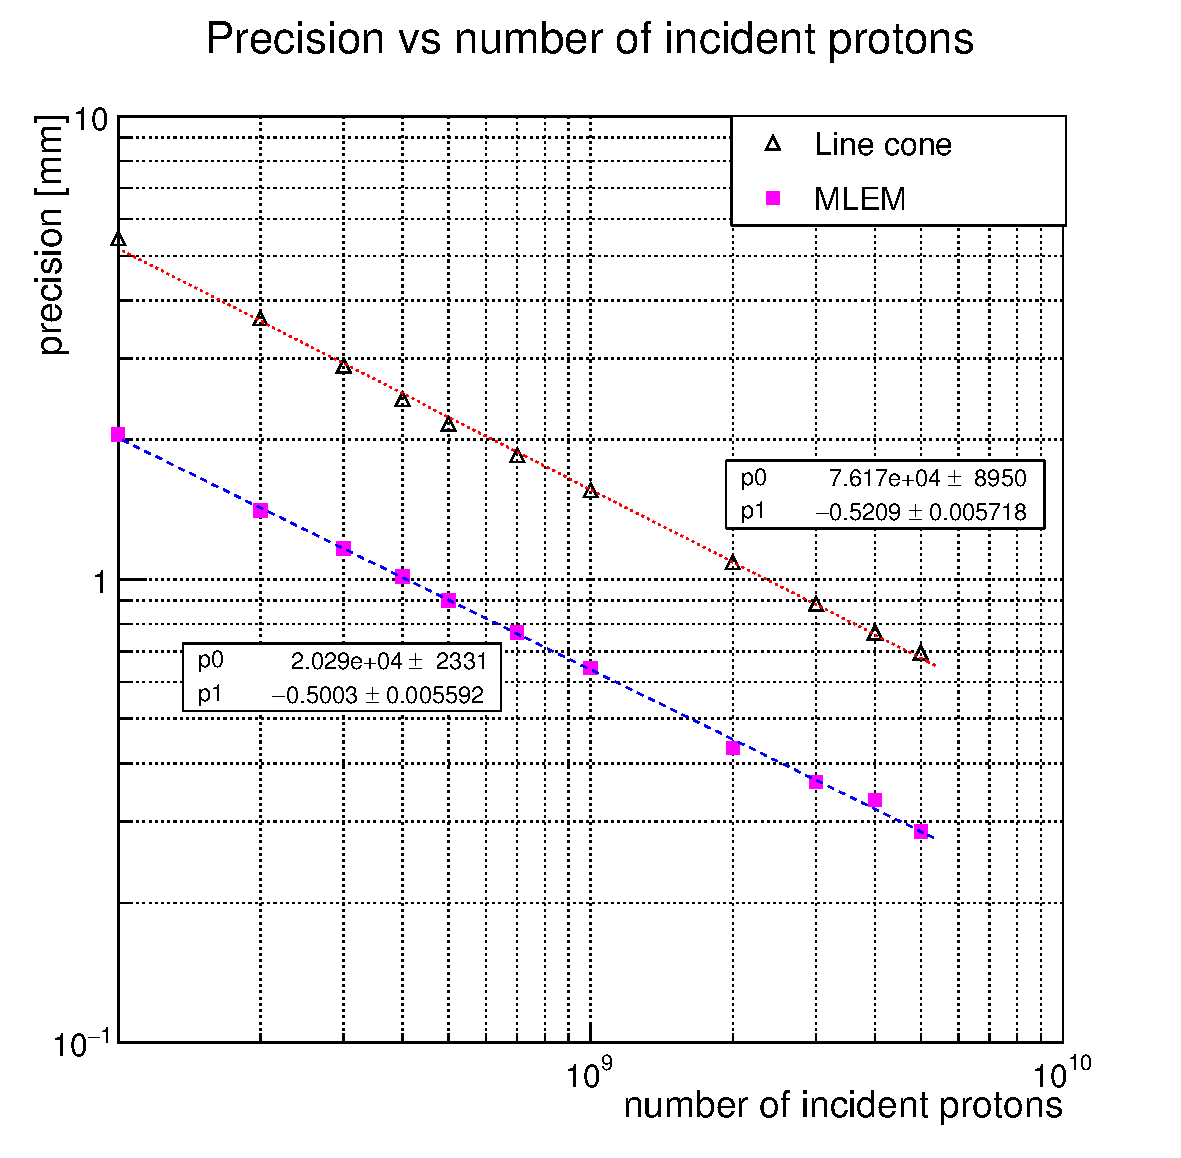
\includegraphics[width=0.7\textwidth]{./Figure/2017-08-02_Precision_Comparaison_linecone_MLEM_Article_Fit.pdf}
\end{figure}



